\newpage
\begin{appendices}
	\section{Intial Project Overview}
		\label{app_ipo}
		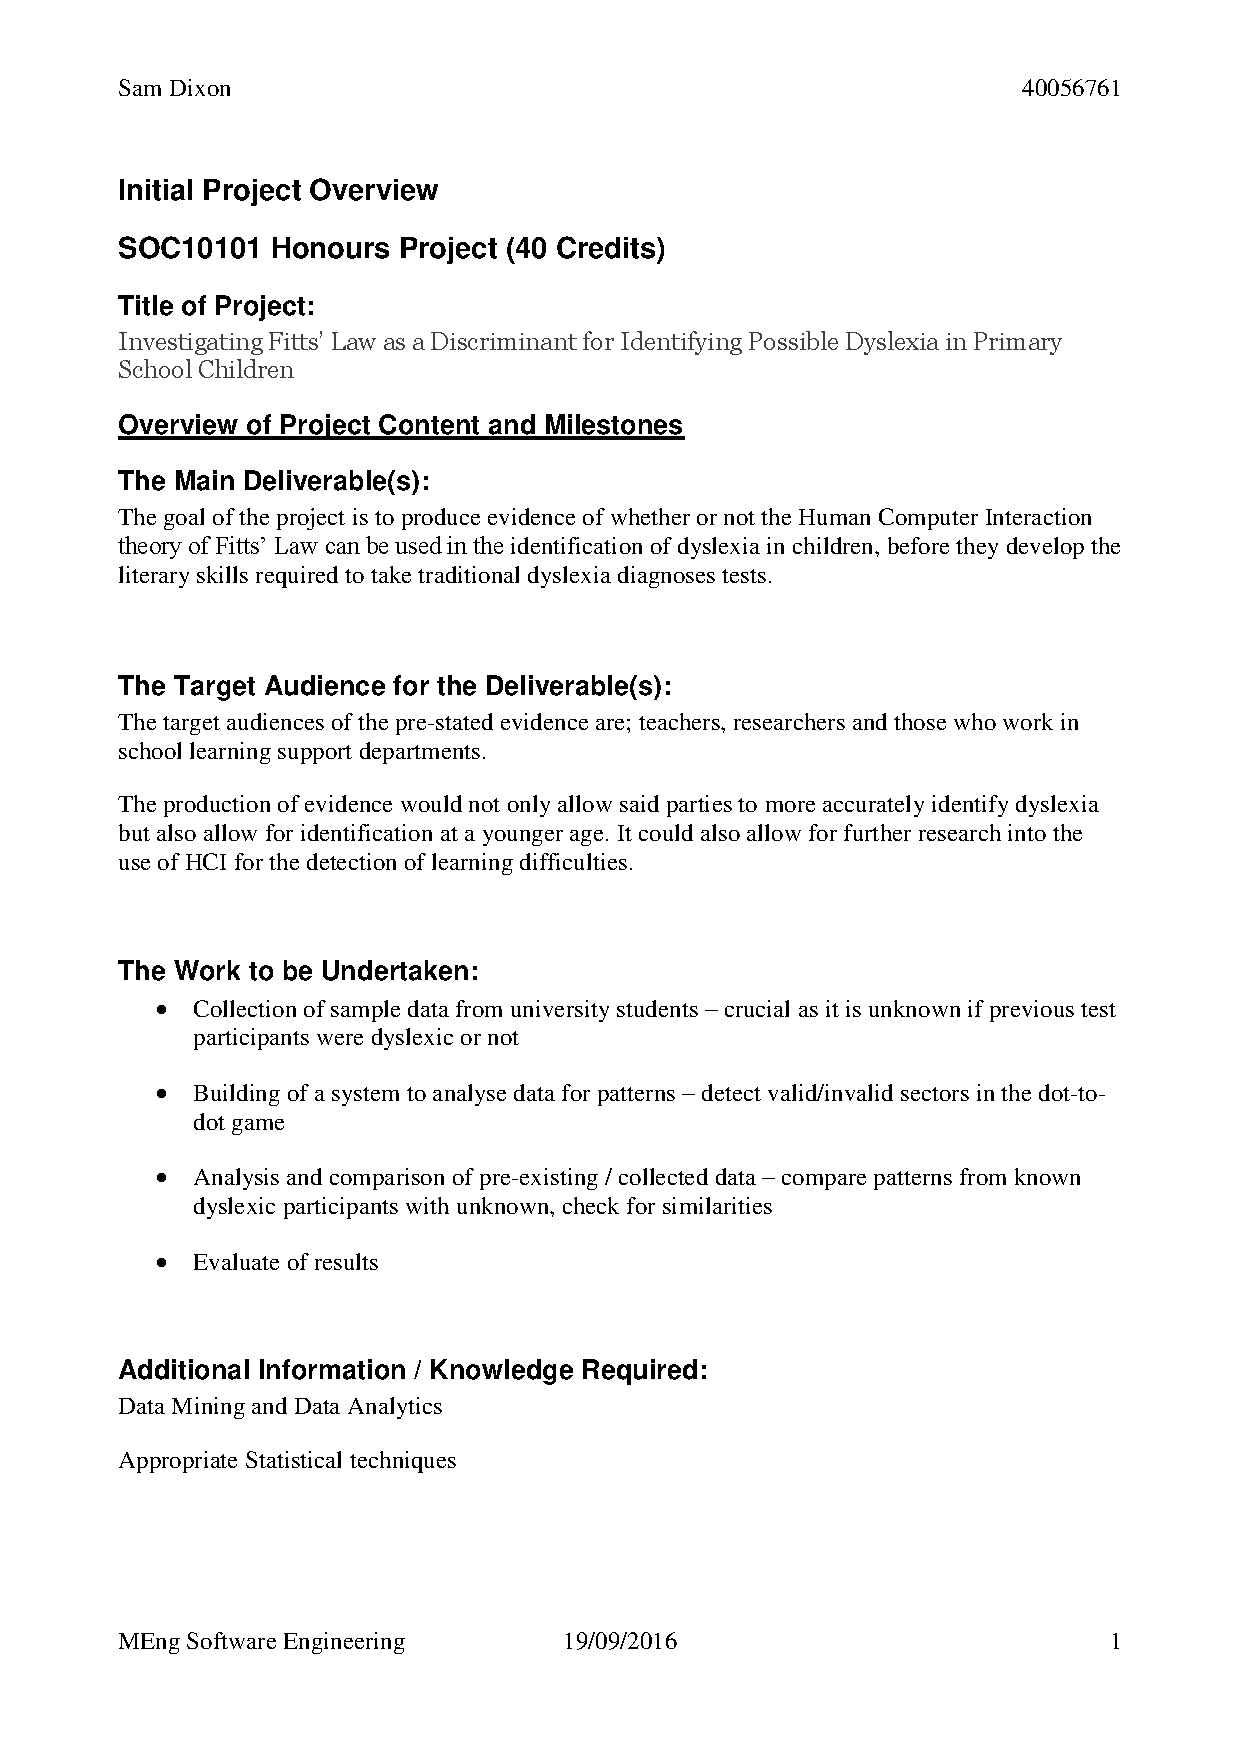
\includegraphics[page=1, width={\textwidth}]{ipo}		
		\includegraphics[page=2, width={\textwidth}]{ipo}
		\newpage
		
	\section{Review Output From}
		\label{app_week9}
		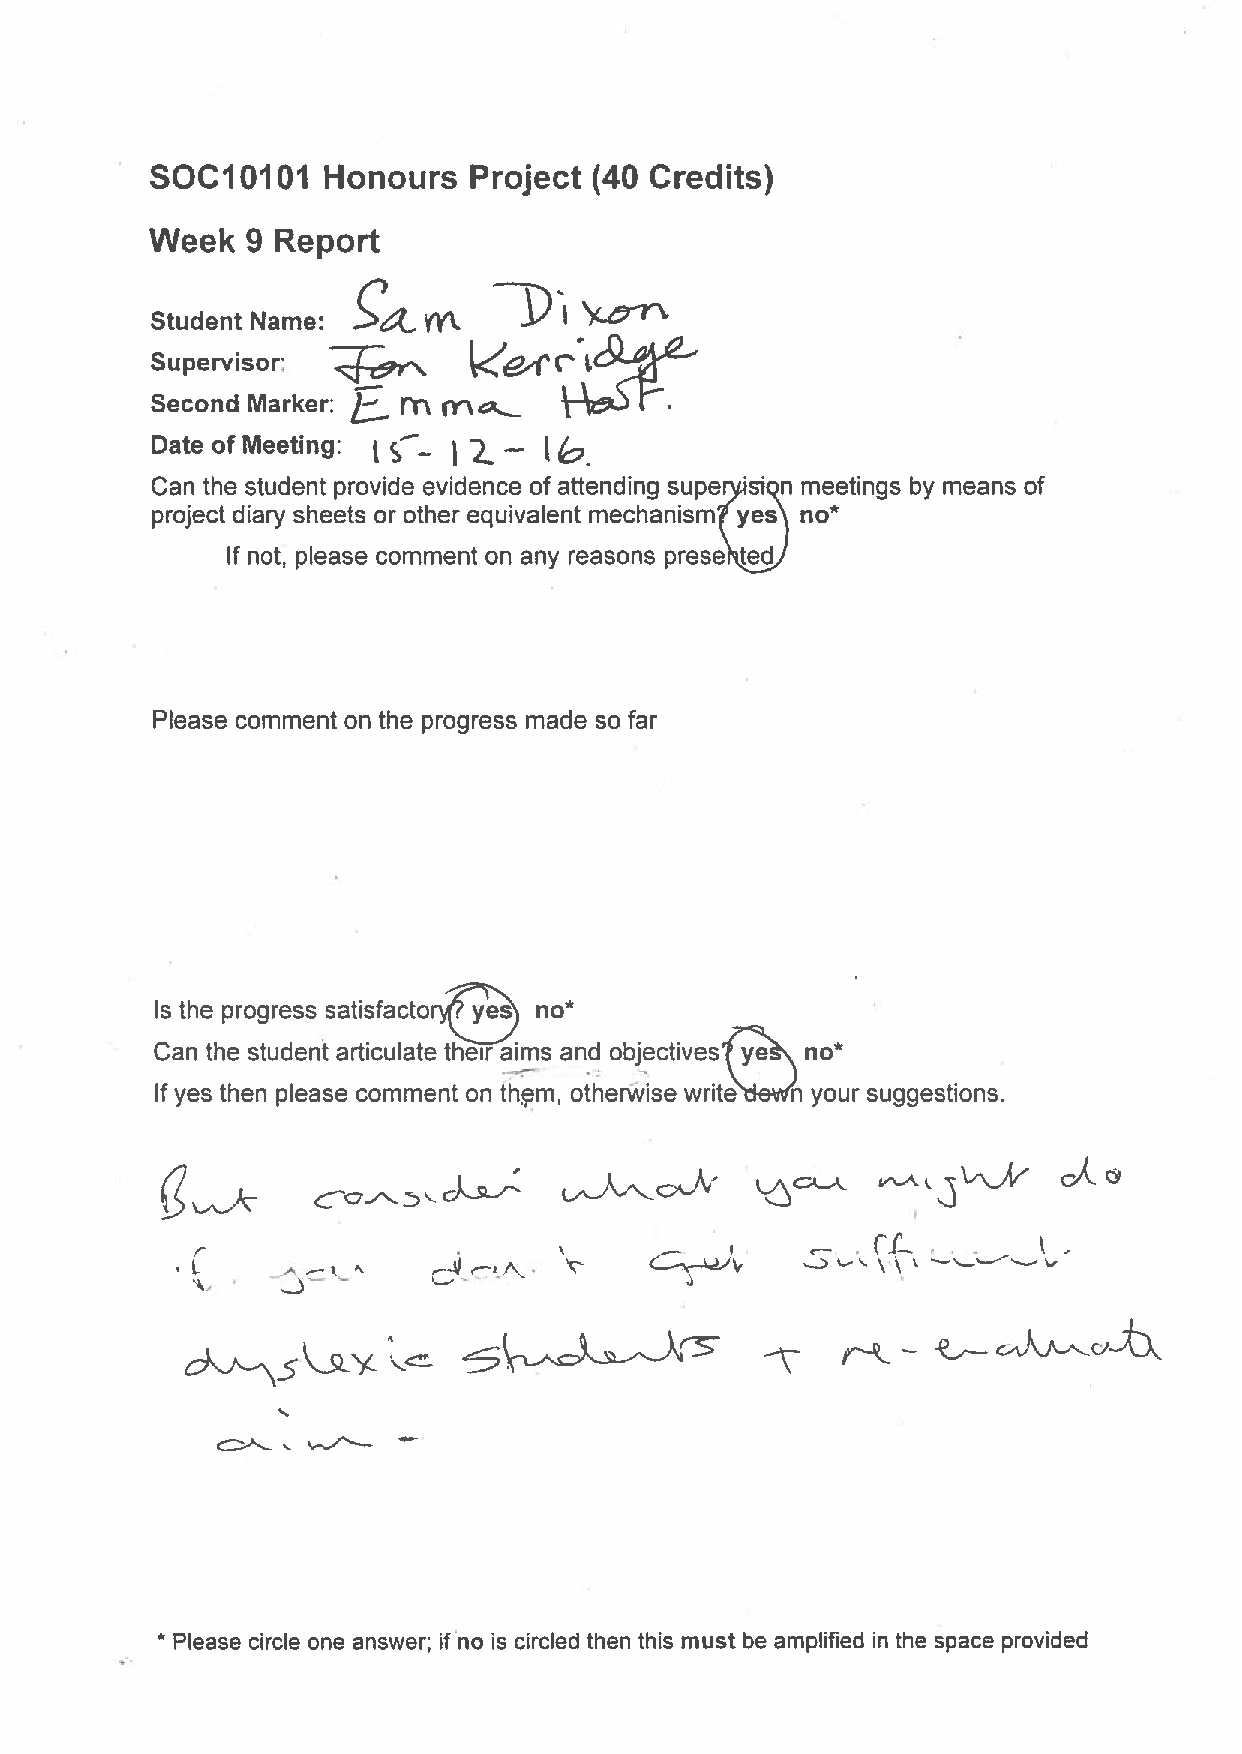
\includegraphics[width={\textwidth}]{midway_a}
		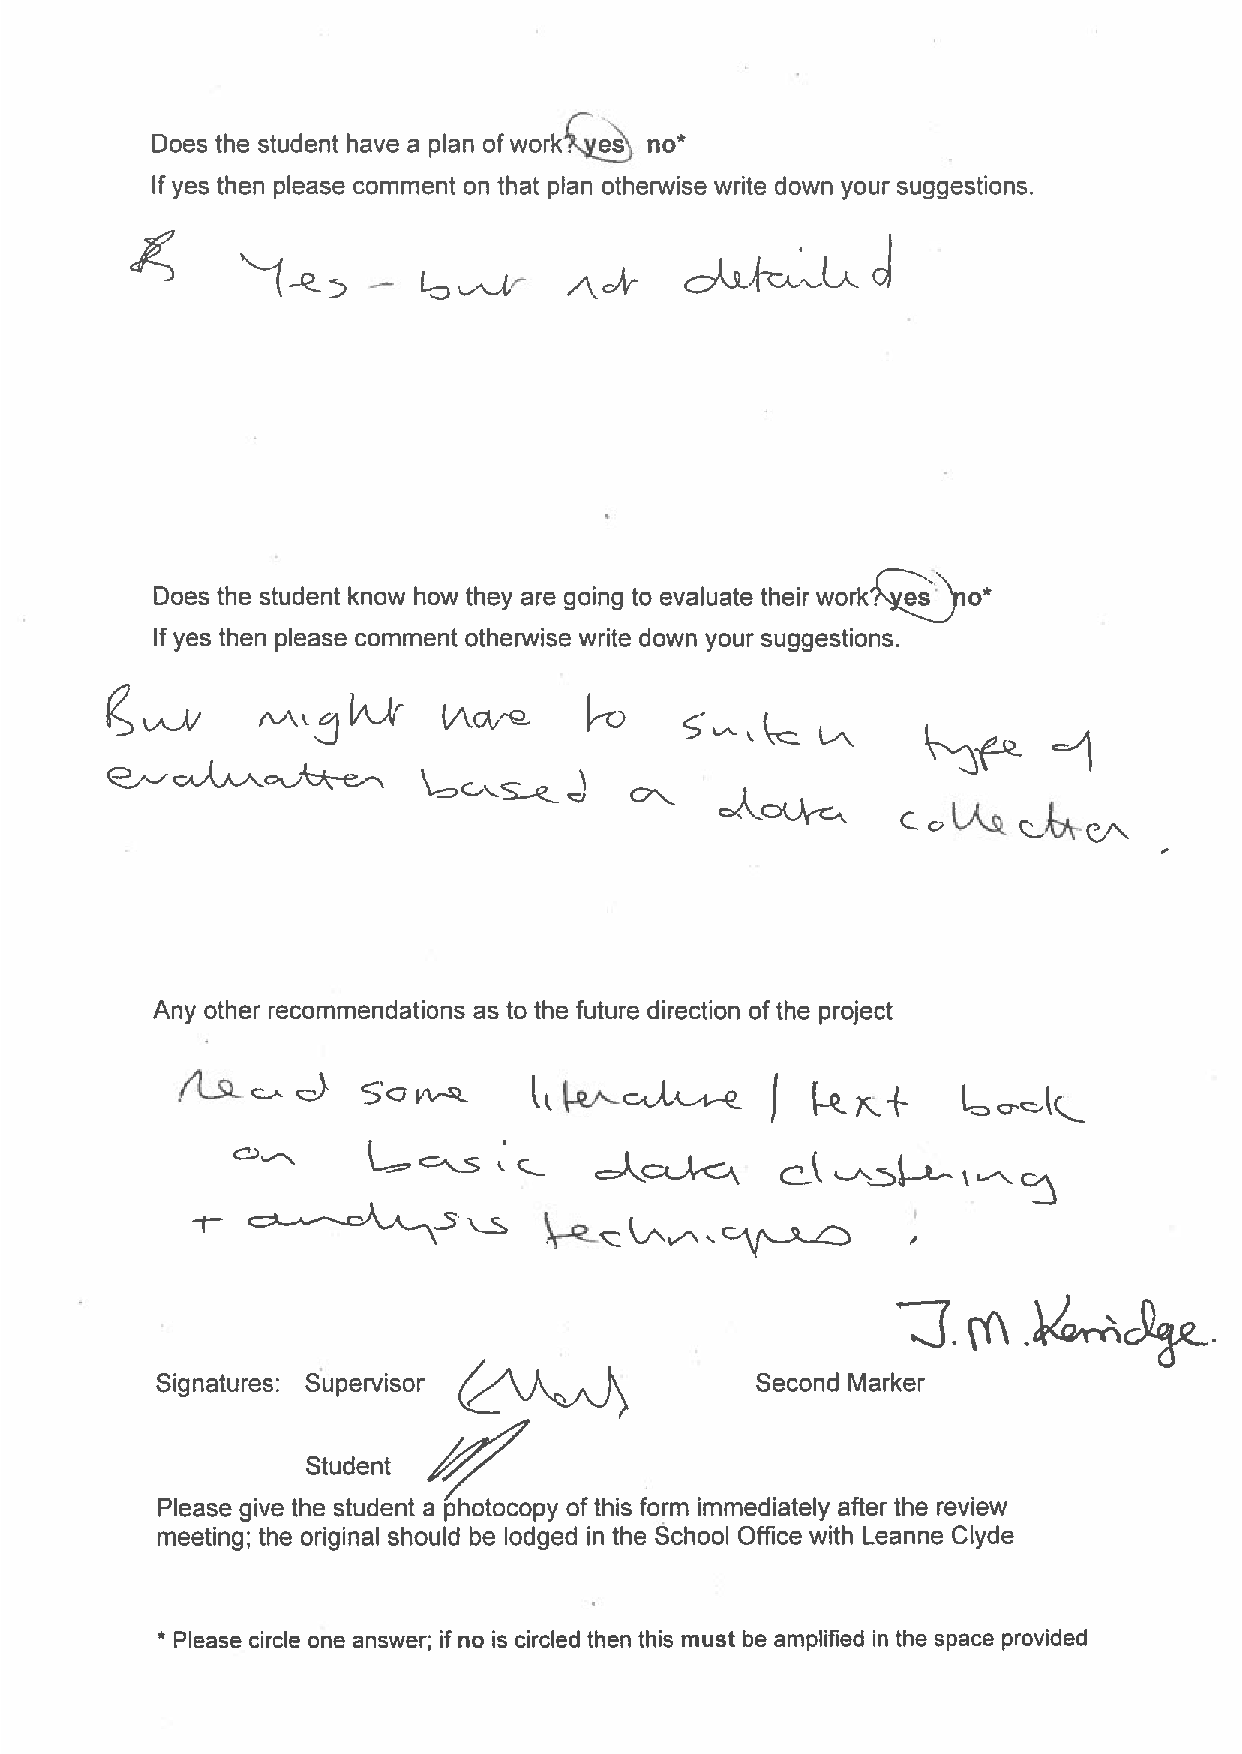
\includegraphics[width={\textwidth}]{midway_b}
		\newpage
		
	\section{Project Blog (Diary Sheets)}
		\label{app_blog}
		\textbf{Captains Log, Stardate 07/09/2016. 07/09/16.}
		Starting to begin my Honours project proper. I have been asked to keep a blog to allow my supervisor to easily keep track of progress.
		The official title of the honours project is:
		“Investigating Fitts Law as a Discriminant for Identifying Possible Dyslexia in Primary School Children”
		Being dyslexic myself, I have keen interest in the processes of identifying dyslexia, and when I found out that one of my lectures was also studying the area, I jumped at the opportunity.
		Lets get learning.\\
		
		\textbf{Week 3-4 Update. 27/09/16.}
		Week 3:
		Hell of a week; Apparently there had been some confusion in the School office, and my Honours registration form had been misplaced, long story short; I spent most of the week trying to sort out admin issues, meaning I got basically no work done for any of my modules, great start to the semester.
		Week 4:
		Working with Jon data and code base. I had previously had all this stuff set up, but my laptop came down with a bad case of Windows 10, and I was forced to reformat. Managed to get the data base reconfigured, and got some code to compile.
		I was originally using Eclipse as my Java IDE, but over the summer I got very attached to IntelliJ and I have been able to port Jon’s project over without much issue.
		The goal for this week is to write some code to identify good/bad sectors in each test and then analyse the valid ones.
		A “bad” sector is one that has a break, pause or loop in it (see the beautiful picture in the header).
		The admin issues should be resolved this week and I will be able to produce some data.
		Here’s hoping.\\
		
		\textbf{Week 5. 06/10/16.}
		Hectic week once again, I have started a group project in one of my modules, so a lot of my time was spent organising that.
		Below is a more accurate representation of what determines a valid sector.
		I also read some more papers on Fitts’ models, the basic formula of calculating the difficulty between two points is: [picture]
		Pretty basic once you have it on paper.
		I am still trying to extract only valid sectors from Jon’s data set, but once I have them it should be clear sailing to calculate their Fitts’ score.
		Lets hope that next week is less busy, so I can get my head down and blast through some work.\\
		
		\textbf{Week 6. 13/10/16.}
		A hectic week once again, no rest for the wicked.
		The current goal is to extract all the valid sectors from the data base, which first requires me to find all the invalid ones. To achieve this I have cobbled together a very basic python script, that loops through all the invalid events (loops, lifts, pauses), gets the coordinate of the event and then assigns the row with the appropriate sector number.
		As can be seen, I have appended the sector ID to the end of each list, a simple process that will prove invaluable later.
		Once I have compiled my list invalid sectors, extractor the valid ones will be a piece of\\
		
		\textbf{Week 7. 20/10/16.}
		We are close, really, REALLY close.
		
		After a week of tinkering I can now produce a list of  every collection, and all the invalid sectors within it.
		Now that we have all the bad sectors named and shamed, pulling the valid ones will be super simple.
		I am quite annoyed I wasnt able to get the final iteration of this program complete before my supervisor meeting, but considering how close I am I cannot be too upset.
		Onwards to next week, and some proper data.
		\\
		
		\textbf{Week 8. 27/10/16.}
		So. Didnt manage to get much work this week due to my other modules getting in the way.
		I was however able to test the results of my last weeks work, by comparing my script’s output to images of the pattern’s drawn by the children.
		My script believes that the child in the image made mistakes in sectors {1, 3, 4, 5, 6}. If we look at the image above, we can see that this is accurate.
		There is some noise in a lot of the images, but from what I can tell my script is producing valid results, which is nice.
		Plan for next week: actually focus on my honours and get some more code done.\\
		
		\textbf{Week 9. 03/11/16.}
		This week turned out similar to the last, with very little work being done on my honours project.
		I have two deadlines for other modules this week, Friday and Sunday – once I have completed these assessments I will have mountains of time to spend on this project.
		I quite annoyed that I haven’t been able to spend any time on my honours, as it is significantly more interesting than some of the other work I am doing.
		Till next week!\\
		
		\textbf{Week 11. 17/11/2016.}
		Real life Strikes once again.
		Working away on my progress report for my second marker.
		Looking forward to getting this finished and back to development.
		Onwards and upwards.\\
		
		\textbf{Week 12. 24/11/2016.}
		Finally got my progress report into my second marker, hooray!
		Other than that, I am focusing mostly on upcoming coursework and exams.
		I have done a little poking around with the data i generated, but I am yet to find anything particularly interesting or outlandish – I will have to put aside a few hours for some in depth data analytics.
		I have a meeting with my second marker on the horizon, so I want to prepare for any potential that she may have for me – as well my next steps.\\
		
		\textbf{Trimester 2 - Week 1. 15/01/2017.}
		Back in business.
		Spent a lot of time collecting data from various people at the university – it was good fun.
		I have also had a quick look at said data, and I am trying to see if I can spot any patterns. If I do notice anything common, I need to update my python scripts to also identify it.
		All in all, a great first week back on the project.
		\\
		
		\textbf{Trimester 2 - Week 2. 23/01/2017.}
		Collected some more data from volunteers this week, but many of them did not show up, which was a shame.
		Started work on analysing the data I did collect to create a Regression analysis. but work on it has been slow, and I don’t have anything to show for it as of right now.
		I am also considering modifying the database and analysis engine I created, as I now have more information of the test subjects (whether they are dyslexic or not) and I don’t want to have to swap between MySQL and excel spread sheets to collate information.
		A slow week overall, but ground work has been put down which will allow multiple tasks to be completed this week, namely: regression analysis and Dyslexic / Non-dyslexic comparison.\\
		
		\textbf{Trimester 2 - Week 3. 30/01/2017.}
		We have some Charts!
		Some of the results seem a little skewed – likely due to the difference in numbers between dyslexic and non-dyslexic test participants.
		The data extraction scripts I was previously using had to be completely rewritten, as the new database I am using for University test participants is using a different schema structure from the. This leaves us with a small issue in regards to loop detection – which is still in the process of being reworked.
		More charts, graphs and analytics to come very soon!\\
		
		\textbf{Trimester 2 - Week 4. 06/02/2017.}
		Starting on the writing of the disserstion proper.
		Spent a little time on sorting out a Latex template and have some simple outline paragraphs for each section I am going to write.
		I am going to have my supervisor check over what I have so far to ensure the layout is alright, then I will try to crack out a rough draft of Lit review and methodology.
		I should be running some tests on the SEBE students soon, and more data will make the analysis task all the easier.\\
		
		\textbf{Trimester 2 - Week 5. 13/02/2017.}
		Spent a lot of time this week dealing with other modules, so I did not get as much honours complete as I was hoping – though I did spend some time updating scripts to include loop detection.
		While examining the data produced by the updated scripts, I came across the information above, which seems to indicate that Dyslexic participants struggle with sector 8 the most, for pattern 4 at least.
		Will examine similar data further during the week, to see if I can quantify this claim any further.\\
		
		\textbf{Trimester 2 - Week 6. 20/02/2017.}
		No picture this week!
		Been working on extracting as many varibles as possible from the data, as well as combining  trhough B’s data – has taken a long time but is going well.
		I have spent a lot of time trying to prove and quantifying my data – hence no pictures this week, once I prove that my results are valid, we will have graphs-galore!
		Plan is to keep working with B’s and my own data, and get as much varibles as possible in order to do some pattern mathcing.\\
		
		\textbf{Trimester 2 - Week 8. 06/03/2017.}
		Playing with data and making some charts.
		Most of the charts are fairly nondescript, mainly because I forgot to update the database before my analysis.
		I am reproducing the charts asap, with the correct data, and we will see if they make anymore sense.\\
		
		\textbf{Trimester 2 - Week 10. 20/03/2017.}
		Not a hugely productive week overall – mainly due to other courseworks and my initial work on the poster.
		I was looking at the “key-sectors” – areas that had large difference between dyslexic/non-dyslexic participants.
		Both the sectors I am interested in are upward slopes of similar angles/lengths – but other sectors of similar proportions do not have as large differences.
		I am using these two sectors as “anchors” to compare possible dyslexics against.
		I am still parsing through B’s data – it is extremely verbose so I am trying to figure out which data I actually need and what can be ignored.
			
	\section{Dot-to-Dot Task Participant Permission Form}
		\label{app_permission}
		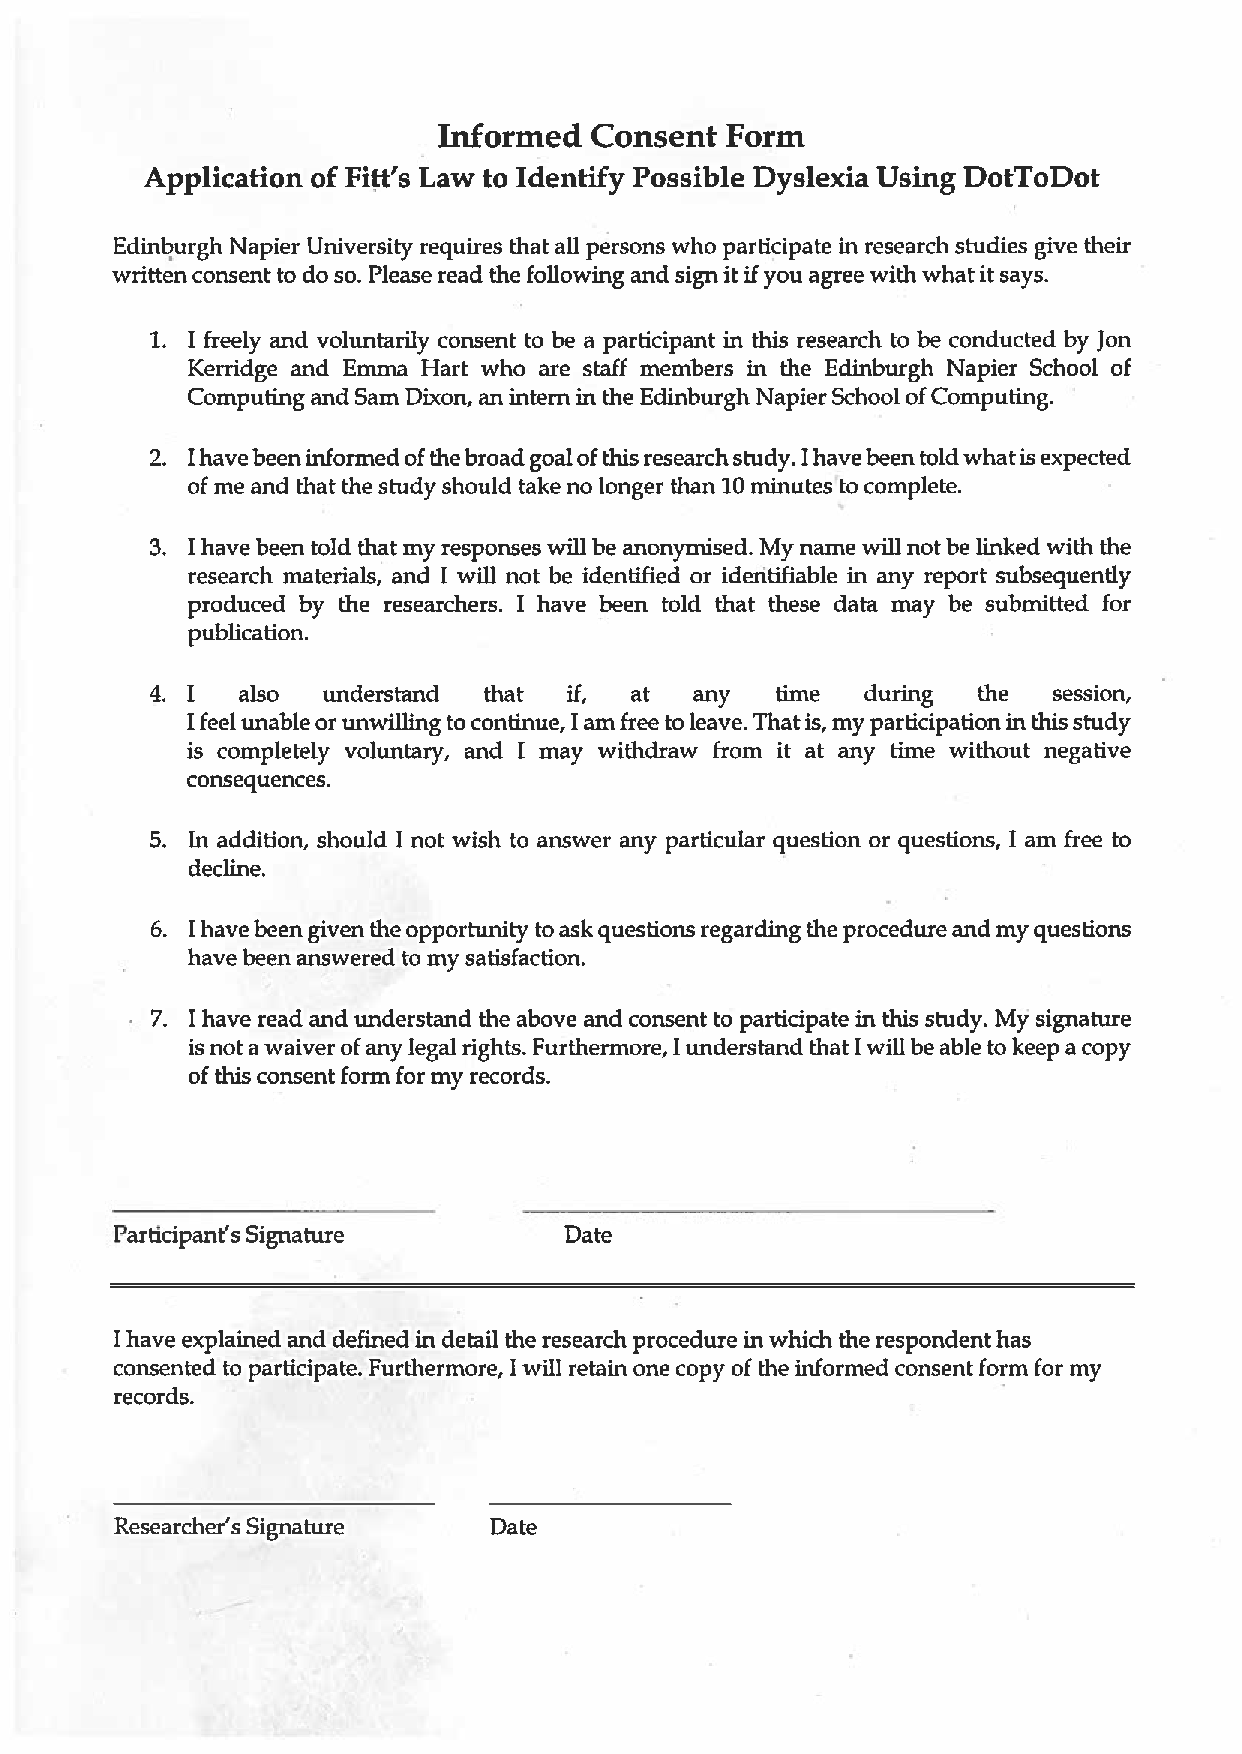
\includegraphics[width={\textwidth}]{dtd_permission}
		
	\section{Movement Time Regression Analysis}
		\label{app_reg}
		\begin{table}[h]
			\centering
			\caption{Pattern 3 - Regression Analysis input data.}
			\label{tab_pat_3_reg}
			\begin{tabular}{|c|c|}
				\hline
				\textbf{Sector ID} & \textbf{Movement Time} \\ \hline
				2.00               & 654.01                 \\ \hline
				3.59               & 1127.17                \\ \hline
				3.75               & 1073.18                \\ \hline
				4.04               & 1269.22                \\ \hline
				4.15               & 1334.30                \\ \hline
				4.26               & 1500.22                \\ \hline
				4.43               & 1991.61                \\ \hline
			\end{tabular}
		\end{table}
		
		\begin{table}[h]
			\centering
			\caption{Pattern 4 - Regression Analysis input data}
			\label{tab_pat_4_reg}
			\begin{tabular}{|c|c|}
				\hline
				\textbf{Sector ID} & \textbf{Movement Time} \\ \hline
				3.32               & 1000.80                \\ \hline
				3.48               & 1119.50                \\ \hline
				3.61               & 1105.89                \\ \hline
				3.68               & 1584.11                \\ \hline
				3.68               & 1132.42                \\ \hline
				3.82               & 1219.60                \\ \hline
				3.82               & 1187.48                \\ \hline
				3.97               & 1216.46                \\ \hline
			\end{tabular}
		\end{table}
		
	\section{Code and Data Listings}
		Due to the sensitive nature of personal data, code and data listings were omitted from this dissertation to adhere with Data Protection laws and Ethical agreements. Samples of code and data are available within the media device submitted with this dissertation, and further disclosure can be made available upon request.
		
	\section{Non-Dominant Hand Results}
		Throughout this dissertation, charts depicting the \(MT\), \(IP\), and similar are presented to provide aid in the visualisation of results. The previously mentioned charts all depict data collected from participants dominant hands. The non-Dominant hand equivalent charts are presented here.
		
		\begin{figure}[!htb]
			\centering
			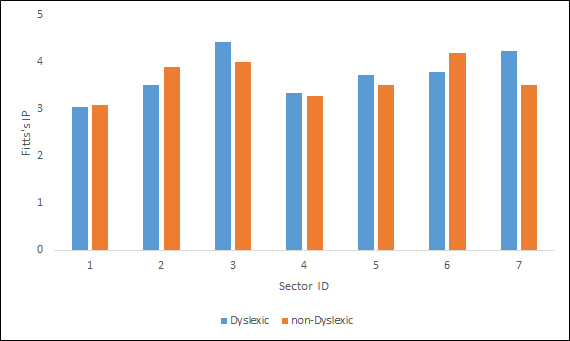
\includegraphics[width = \textwidth]{pat_3_ip_val_ndom}
			\caption{Average Fitts's \(IP\) for pattern 3 sectors without errors, executed with the non-dominant hand.}
			\label{fig_pat_3_ip_ndom}
		\end{figure}		
		
		\begin{figure}[!htb]
			\centering
			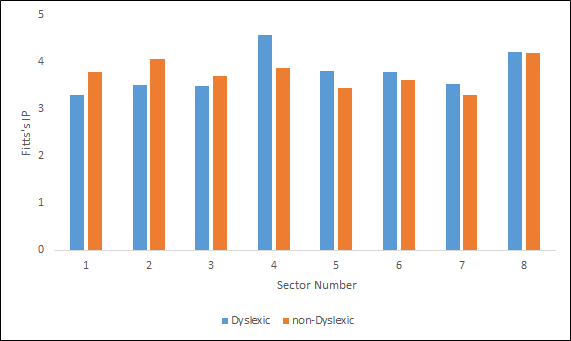
\includegraphics[width = \textwidth]{pat_4_ip_val_ndom}
			\caption{Average Fitts's \(IP\) for pattern 4 sectors without errors, executed with the non-dominant hand.}
			\label{fig_pat_4_ip_ndom}
		\end{figure}
	
	\begin{figure}[!htb]
		\centering
		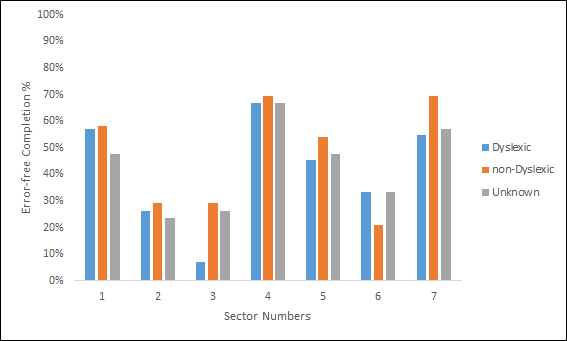
\includegraphics[width = \textwidth]{pat_3_com_ndom}
		\caption{Pattern 3 - Average sector completion rate with no errors, executed with the non-dominant hand.}
		\label{fig_pat_3_com_ndom}
	\end{figure}		
	
	\begin{figure}[!htb]
		\centering
		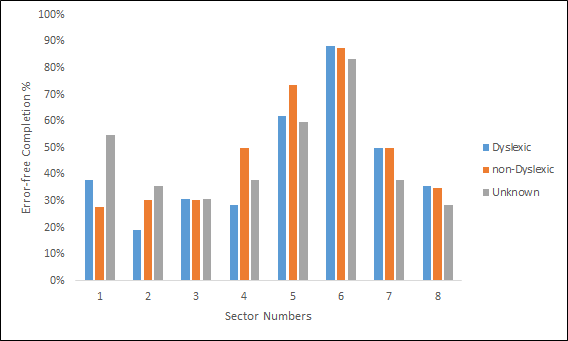
\includegraphics[width = \textwidth]{pat_4_com_ndom}
		\caption{Pattern 4 - Average sector completion rate with no errors, executed with the non-dominant hand.}
		\label{fig_pat_4_com_ndom}
	\end{figure}
	
\end{appendices}